\chapter{Architektura}
\label{cha:architektura}
Na podstawie analizy możliwych rozwiązań sprzętowych w~rozdziale \ref{cha:specyfikacja} oraz przedstawionych poniżej założeń architektury platformy dokonano wyboru urządzeń, które będą stanowiły część sprzętową tworzonego interfejsu.

\section{Założenia architektury sprzętowej}
Aby wybrać odpowiedni dla przygotowywanego prototypu interfejsu zestaw urządzeń, określone zostały założenia i~wymagania, jakie urządzenia powinny spełniać:
\begin{enumerate}
\item Urządzenie powinno być lekkie, aby używanie go przez gracza nie powodowało dyskomfortu, który może wpłynąć negatywnie na jakość odbieranych danych.
\item Dokładność sensorów dostępnych w~urządzeniu powinna być jak największa, aby mieć pewność odczytywanych zachowań użytkownika.
\item Urządzenie powinno być łatwe w~obsłudze, zarówno w~kwestii jego zamontowania, jak i~uruchomienia odczytów. Powinno być także jak najmniej inwazyjne podczas pomiaru, aby zminimalizować dyskomfort użytkownika.
\item Dla wybranego urządzenia powinno być dostępne oprogramowanie umożliwiające odczyt pomiarów w~wybranym środowisku do tworzenia gier. Najlepiej, gdyby rozwiązanie było dostępne w~postaci biblioteki oferowanej przez twórcę sprzętu, lub rozszerzenia silnika, które umożliwi odczyt danych z~urządzenia.
\item Urządzenie powinno mieć możliwość połączenia bezprzewodowego, najlepiej przy pomocy technologii Bluetooth, lub innego protokołu umożliwiającego bezprzewodowy odczyt pomiarów z~urządzenia.
\item Przynajmniej jedno z~urządzeń powinno umożliwiać odczyt pracy serca, w~postaci pomiaru pulsu lub elektrokardiogramu. Pomiar pracy serca jest jedną z~podstawowych metod umożliwiających określenie zmiany w~stanie emocjonalnym użytkownika.
\item Przynajmniej jedno z~urządzeń powinno umożliwiać pomiar ruchów mięśni. Odczytane sygnały mogą być wykorzystane do wpływania na rozgrywkę w~zależności od aktywności mięśniowej użytkownika w~danej partii ciała.
\end{enumerate}


\section{Garmin HRM-Run}
Krótko o~urządzeniu, co odczytujemy, dlaczego to a~nie n.p. BITalino
\begin{figure}
	\centering
	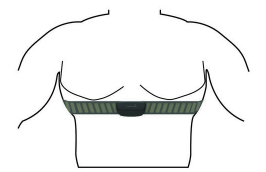
\includegraphics[width=0.5\linewidth]{images/garmin_hrm_placement.png}
	\caption{Miejsce montażu czujnika tętna Garmin HRM-Run, źródło:~\cite{garmin_manual}}
	\label{fig:garmin_placement}
\end{figure}

\section{BITalino Revolution Kit}
Krótko o~urządzeniu i~możliwościach, dlaczego tylko EMG (elektrody, nadmiar kabli, ogólne wady i~zalety)
\begin{figure}
	\centering
	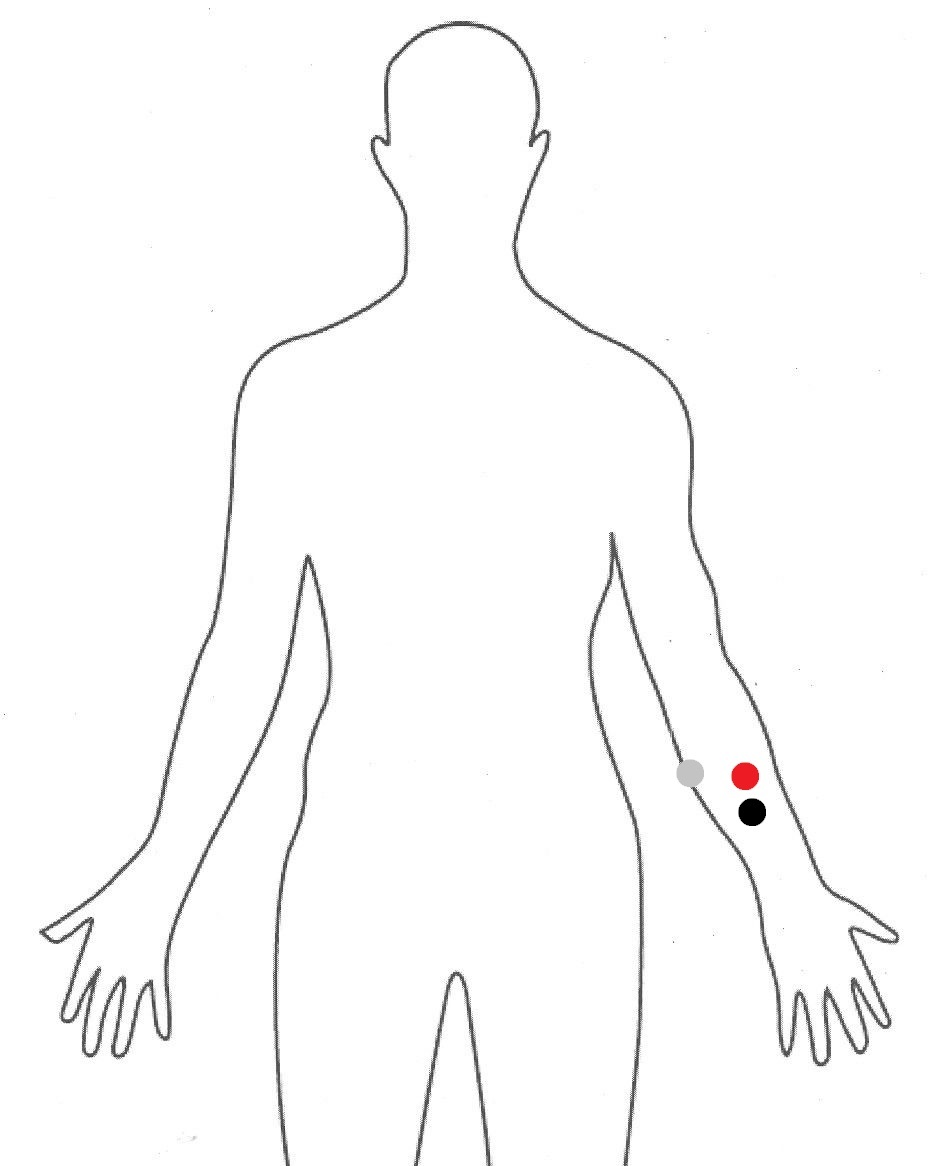
\includegraphics[height=0.3\textheight]{images/bitalino_placement.jpg}
	\caption{Sposób przypięcia elektrod dla sensora EMG,  kolor czerwony oznacza elektrodę dodatnią, czarny ujemną, a~szary elektrodę referencyjną}
	\label{fig:bitalino_placement}
\end{figure}

\section{Dualshock 4}
krótko o~urządzeniu, wykorzystanie akcelerometru do odczytu pobudzenia gracza
